\documentclass[11pt,a4paper]{article}

\usepackage{iftex}
\ifPDFTeX
  \usepackage[utf8]{inputenc}
  \usepackage[T1]{fontenc}
  \usepackage{lmodern}
\else
  \usepackage{fontspec}
\fi
\usepackage[turkish]{babel}
\usepackage[margin=2.4cm]{geometry}
\usepackage{microtype}
\usepackage{amsmath,amssymb}
\usepackage{graphicx}
\usepackage{booktabs,tabularx,array}
\usepackage{enumitem}
\usepackage{placeins}
\usepackage[hidelinks]{hyperref}
\hypersetup{pdftitle={NeuroDino: Chrome T-Rex Oyununu Oynayan Küçük Bir Sinir Ağının Nöroevrimle Eğitimi, Davranış Analizi ve İyileştirilmesi}, pdfauthor={Ahmet Şafak Yıldırım}, pdflang={tr}}

\setlength{\parindent}{0pt}
\setlength{\parskip}{0.45em}
\setlist[itemize]{leftmargin=*,itemsep=0.25em,topsep=0.25em}
\setlist[enumerate]{leftmargin=*,itemsep=0.3em,topsep=0.25em}
\newcolumntype{Y}{>{\raggedright\arraybackslash}X}

\title{\textbf{NeuroDino: Chrome T-Rex Oyununu Oynayan Küçük Bir Sinir Ağının Nöroevrimle Eğitimi, Davranış Analizi ve İyileştirilmesi}}
\author{Ahmet Şafak Yıldırım\\[0.5em]
\small Kod, model ve canlı demo: \url{https://github.com/ahm3texe/NeuroDino}}
\date{Aralık 2025; gözden geçirilmiş sürüm Ekim 2026}

\begin{document}
\shorthandoff{=}
\maketitle

\begin{abstract}
Bu çalışmada Chrome T-Rex Runner oyununu oynayan küçük bir sinir ağı genetik algoritmayla eğitilmiş ve davranışı ölçülmüştür. Ajan, oyun durumunu özetleyen 12 girdiyi 12--48--3 yapısında tam bağlı bir ağla (771 parametre) zıpla, eğil ve koş eylemlerinden birine dönüştürür. Her nesilde aynı bölümü oynayan 50 bireylik popülasyon 6,55 saatte 83 nesil evrilmiş ve 547.287 puanlık bir rekor kırmıştır. 200 yeni oyunda ağ, eğitimdeki oyun döngüsünde oyunların \%97,5'inde maksimum hıza ulaşmış ve \%55'inde 4 saati tamamlamıştır. Ağın kararını bir kare daha güncel bilgiyle verdiği web sürümünün döngüsünde ise oyunların \%56,5'i maksimum hıza ulaşmadan bitmiş, ulaşanlar neredeyse hiç ölmemiştir. Ölüm anlarının geometrisi ve girdi ablasyonu, başarının zıplamanın yaklaşık bir karelik zamanlamasına bağlı olduğunu göstermektedir; ağ hiç eğilmemekte ve 12 girdiden altısının sıfırlanması hiçbir oyunun sonucunu değiştirmemektedir. Web sürümünün döngüsünde ve her bireyin 10 oyunda değerlendirildiği bir düzenle 40 nesil (57 dakika) yeniden eğitilen v2, 200 test oyununun hepsinde maksimum hıza ulaşmış ve 190'ında 4 saati tamamlamıştır. v2'nin test oyunlarındaki 10 ölümünün hepsinde dino, bir sonraki engel için zıplaması gerektiğinde hâlâ havadadır ve havada eğilerek hızlı düşmek hepsini önleyebilirdi. v2'ye yalnızca eğil çıkışını besleyen 8 nöron eklenmiş ve bu nöronlar, iki seçeneğin de oyunda denenmesiyle etiketlenen karelerden gradyan inişiyle eğitilmiştir. Elde edilen v3, hiçbir modelin oynamadığı 1.000 dört saatlik oyunda v2'nin 40 ölümüne karşı 3 kez ölmüştür. Kod, modeller, bütün değerlendirme oyunları ve herkesin aynı oyunu canlı izlediği deterministik bir web sürümü açık olarak paylaşılmıştır.

\textbf{Anahtar Kelimeler:} Nöroevrim; genetik algoritmalar; yapay sinir ağları; girdi ablasyonu; oyun ajanları; Chrome T-Rex.
\end{abstract}

\section{Giriş}

Video oyunları, kontrollü ve tekrarlanabilir dinamik ortamlar sundukları için yapay zekâ yöntemlerini sınamakta sıkça kullanılır; derin pekiştirmeli öğrenmenin Atari oyunlarındaki başarısı bunun bilinen bir örneğidir \cite{mnih2015}. Basit kurallarına karşın hızlı tepki ve hassas zamanlama gerektiren sonsuz koşu oyunları da gerçek zamanlı karar vermeyi incelemek için elverişlidir.

Gradyan tabanlı pekiştirmeli öğrenmeye bir alternatif, ağ ağırlıklarının evrimsel yöntemlerle doğrudan optimize edildiği nöroevrimdir. Genetik algoritmaların ve evrim stratejilerinin derin ağlarda bile pekiştirmeli öğrenmeyle rekabet edebildiği gösterilmiştir \cite{such2017,salimans2017}. Ödülün yalnızca bölüm sonunda alındığı ve girdilerin az sayıda olduğu problemlerde, küçük bir ağın ağırlıkları gradyan hesaplamadan aranabilir.

Bu çalışmada Chrome T-Rex Runner oyunu için bir eğitim ortamı kurulmuş, küçük bir sinir ağı genetik algoritmayla eğitilmiş ve eğitilen ajanın ne yaptığı ve neden öldüğü ölçülmüştür. Katkılar şunlardır:
\begin{itemize}
  \item Chromium'daki oyunun Python ve Pygame'e aktarılması ve tarayıcı gerektirmeyen bir eğitim ortamı;
  \item 12 girdili, 771 parametreli bir ağın genetik algoritmayla eğitimi ve eğitim sürecinin kayıtlarla ayrıntılı analizi;
  \item eğitilen ajanın 200 yeni oyunda, eğitimdeki ve demodaki iki farklı oyun döngüsüyle değerlendirilmesi, ölüm nedenlerinin incelenmesi ve hangi girdileri kullandığının ablasyonla ölçülmesi;
  \item bulunan sorunun eğitim düzeneğinde giderildiği ve sağlamlığı ölçülerek seçilen ikinci bir model (v2);
  \item v2'nin kalan ölümlerinin nedenini bulan bir analiz ve onları, v2'nin zıplamalarına dokunmadan, eklenen nöronlarla büyük ölçüde gideren üçüncü bir model (v3);
  \item herkesin aynı oyunu aynı anda izlediği ve ağın etkinliklerini canlı gösteren deterministik bir web sürümü.
\end{itemize}

\section{İlgili Çalışmalar}

Genetik algoritmalar Holland'ın çalışmasına dayanır \cite{holland1975}; ileri beslemeli ağların ağırlıklarının genetik algoritmayla eğitilmesi ilk olarak Montana ve Davis tarafından gösterilmiştir \cite{montana1989}. Yao, ağırlıkların, topolojinin ve öğrenme kurallarının evrimini kapsayan bir derleme sunar \cite{yao1999}. NEAT gibi yöntemler topolojiyi de evrim boyunca büyütürken \cite{stanley2002}, bu çalışmadaki genetik algoritma topolojiyi değiştirmez, yalnızca ağırlıkları ve bias değerlerini evriltir (v3'e nöronlar elle eklenmiştir). Ölçek tarafında, evrim stratejilerinin \cite{salimans2017} ve basit bir genetik algoritmanın \cite{such2017} milyonlarca parametreli ağları eğitebildiği gösterilmiştir. Bu çalışmadaki ajan ise piksel yerine elle tasarlanmış 12 özellik kullanır ve ağ yalnızca 771 (v3'te 899) parametrelidir.

Eğitilen ajanın davranışını açıklamak için girdilerin kaldırılmasına dayanan ablasyon kullanılmıştır. Bir girdinin çıkarıldığında modelin çıktısını ne kadar değiştirdiğine bakan bu yaklaşım, \cite{covert2021}'de birçok açıklama yöntemini kapsayan ortak bir çerçeve olarak ele alınmıştır.

\section{Materyal ve Yöntemler}

\subsection{Oyun Ortamı}

Chromium'daki T-Rex Runner oyununun TypeScript kaynakları \cite{chromium} Python ve Pygame'e \cite{pygame} aktarılmıştır. Oyunun kuralları korunmuştur: oyun alanı 600$\times$150 pikseldir ve fizik, gerçek zamandan bağımsız olarak saniyede 60 sabit adımla ilerler. Hız saniyede değil kare başına piksel cinsindendir; 6'dan başlar, her karede 0,001 artar ve 7.000. karede 13'e ulaşır. Skor koşulan mesafenin 0,025 katıdır; maksimum hıza yaklaşık 1.662 puanda ulaşılır. Engeller tek tek ya da gruplar halinde gelen küçük ve büyük kaktüslerle, hız 8,5'i geçtikten sonra görülmeye başlayan kuşlardır. Kuşlar üç yükseklikten birinde uçar: $y=50$'deki kuş koşan dinonun üzerinden geçer, $y=75$'teki kuşun altından eğilerek ya da üzerinden zıplayarak geçilebilir, $y=100$'deki kuşun üzerinden zıplanmalıdır.

Çarpışma denetimi de özgün oyundaki gibidir: önce dinonun ve engelin dış kutuları, kesişiyorlarsa her biçime özgü daha küçük kutular karşılaştırılır. Bütün kutular eksenlere hizalıdır; özgün oyun da piksel düzeyinde karşılaştırma yapmaz. İki fark vardır. Eğitim çalıştırıcısı her karede bütün engelleri denetler; özgün oyun yalnızca ilk engeli denetler. Ayrıca özgün oyunun sesli ipucu modu engeller arasındaki boşlukları iki katına çıkarır. Eğitim bu mod kapalıyken, yani normal boşluklarla yapılmıştır; geliştirme sırasında kullanılan Gradio paneli ve izleme betiği ise varsayılan olarak bu modda, yani iki kat boşluklarla çalışmıştır.

Eğitim çalıştırıcısı ile izleme betiği bir karenin adımlarını da farklı sırayla işler. Eğitimde her karede önce ağ, engellerin bir önceki karedeki konumlarına bakarak karar verir; ardından engeller ilerletilir ve çarpışma denetlenir. İzleme betiğinde, Gradio panelinde ve bunlardan aktarılan web sürümünde ise önce engeller ilerletilir, ağ engellerin bu yeni konumlarına bakarak karar verir, ardından çarpışma denetlenir. Böylece aynı ağ, izleme döngüsünde her kararı engelleri bir kare daha yakında görerek verir. Ayrıca eğitimde oyunun gece modu hiç açılmaz. Gece modu yalnızca görseldir, ancak açıkken yıldızlar rastgele sayı çekmediği için oyunun rastgele sayı akışını değiştirir. Bu farkların sonuçlara etkisi Bölüm~\ref{sec:eval}'te ölçülmüştür.

Arayüzsüz modda Pygame sahte bir görüntü sürücüsüyle çalıştırılır ve kare hızı sınırlanmaz; fizik adımı yine 1/60 saniye olduğu için sonuçlar gerçek zamana bağlı değildir. Eğitimde kullanılan sürümde oyun ve panel bu modda da görünmeyen bir yüzeye çizilmeye devam etmiştir. Eğitim kayıtlarındaki zaman damgalarına göre 83 nesil boyunca toplam yaklaşık 8,37 milyon kare 6,55 saatte işlenmiştir: saniyede ortalama yaklaşık 355 kare, yani gerçek zamanın yaklaşık 5,9 katı. En uzun nesilde (77. nesil, yaklaşık 1,69 milyon kare, 63 dakika) bu değer saniyede yaklaşık 445 karedir. Her karede o anda yaşayan bütün ajanlar karar verir.

\subsection{Girdiler}

Ağ ham piksel yerine oyun durumunu özetleyen 12 girdi kullanır (Tablo~\ref{tab:inputs}). Engel girdileri, dinonun önündeki ($x_{\mathrm{engel}} > x_{\mathrm{dino}}$) en yakın iki engel için hesaplanır; engel yoksa ilgili girdiler 0'dır. Mesafeler, oyun hızı arttıkça anlamları değişmesin diye kare cinsinden süreye çevrilir. Çarpışmaya kalan süre girdisi
\begin{equation}
  I_{\mathrm{Dist}} = 1 - \min\!\left(1,\ \frac{x_{\mathrm{engel}} - x_{\mathrm{dino}}}{\max(1, v)\cdot 50}\right)
  \label{eq:tti}
\end{equation}
ile hesaplanır; burada $x_{\mathrm{dino}}$ dinonun sol kenarı, $v$ oyunun kare başına piksel cinsinden hızıdır. Engel 50 kare ya da daha uzaktaysa girdi 0, çarpışmak üzereyse 1'e yakındır. İki engel arasındaki boşluk da aynı biçimde, 15 karelik bir ölçekle çevrilir:
\begin{equation}
  I_{\mathrm{Gap}} = 1 - \min\!\left(1,\ \frac{x_{2} - (x_{1} + w_{1})}{\max(1, v)\cdot 15}\right).
  \label{eq:gap}
\end{equation}
Dinonun yüksekliği, zıplarken $I_{Y} = \min\!\left(1, \max\!\left(0, (y_{\mathrm{zemin}} - y)/30\right)\right)$ olarak verilir (ekran koordinatlarında $y$ aşağı doğru artar), dikey hızı ise $v_y/10$ olarak $[-1, 1]$ aralığına kırpılır; dino yerdeyken ikisi de 0'dır.

\begin{table}[!htbp]
  \centering
  \small
  \caption{Ağın 12 girdisi. Obj1 en yakın, Obj2 ondan sonraki engeldir.}
  \label{tab:inputs}
  \begin{tabularx}{\linewidth}{@{}r l Y l@{}}
    \toprule
    \# & Girdi & Tanım & Aralık \\
    \midrule
    1 & Obj1 Dist & Engele kalan süre, Denklem~\eqref{eq:tti} & $[0, 1]$ \\
    2 & Obj1 Act & Engel $y < 75$ olan kuşsa 1, değilse 0 & $\{0, 1\}$ \\
    3 & Obj1 W & $\min(1,\ \text{genişlik}/75)$ & $[0, 1]$ \\
    4--6 & Obj2 Dist, Act, W & Aynıları, ikinci engel için & \\
    7 & Speed & $v/13$ & $[0{,}46;\ 1]$ \\
    8 & Gap & İki engel arasındaki boşluk, Denklem~\eqref{eq:gap} & $[0, 1]$ \\
    9 & DinoY & Zıplarken zeminden yükseklik / 30, en çok 1 & $[0, 1]$ \\
    10 & DinoVel & Zıplarken dikey hız / 10 (yükselirken negatif) & $[-1, 1]$ \\
    11 & Air & Dino havadaysa 1 & $\{0, 1\}$ \\
    12 & Duck & Dino eğiliyorsa 1 & $\{0, 1\}$ \\
    \bottomrule
  \end{tabularx}
\end{table}
\FloatBarrier

Bu tasarımın üç özelliği bulguları doğrudan etkiler. Birincisi, Act girdisi eğilmeyi gerektiren kuşu işaretlemek amacıyla tasarlanmış olsa da $y < 75$ eşiği yalnızca ${y = 50}$'deki kuşu seçer; bu kuş koşan dinonun üzerinden geçtiği için hiçbir eylem gerektirmez. ${y = 75}$ ve ${y = 100}$'deki kuşların genişliği de aynı olduğundan, ağ bu iki kuşu girdilerinden ayırt edemez. İkincisi, dino zıplarken zeminden yaklaşık 90 piksel yükselir; yükseklik 30'a bölündüğü için DinoY havada geçen sürenin yaklaşık \%85'inde 1'de takılı kalır. Üçüncüsü, bir engel dinonun sol kenarını geçtiği anda, dinoyla hâlâ çakışıyor olabilse de girdilerden çıkar.

\subsection{Yapay Sinir Ağı}

Ağ 12 giriş, 48 gizli ve 3 çıkış nöronundan oluşan, tam bağlı ileri beslemeli bir ağdır. Girdi vektörü $\mathbf{x}\in\mathbb{R}^{12}$ için
\begin{align}
  \mathbf{h} &= \tanh(\mathbf{W}_{ih}\mathbf{x}+\mathbf{b}_{h}),\\
  \mathbf{y} &= \operatorname{softmax}(\mathbf{W}_{ho}\mathbf{h}+\mathbf{b}_{o})
\end{align}
hesaplanır ve ajan en yüksek olasılıklı eylemi, $\operatorname*{arg\,max}(\mathbf{y})$, uygular. Ağın $12\times48 + 48\times3$ ağırlığı ve $48 + 3$ bias değeri, yani toplam 771 parametresi vardır (v3'e eklenen 8 nöron Bölüm~\ref{sec:v3}'da anlatılmıştır); hesaplamalar NumPy \cite{numpy} ile 64 bit kayan noktada yapılır. Ağırlıklar Glorot (Xavier) yöntemine göre \cite{glorot2010}
\begin{equation}
  W \sim U\!\left(-\sqrt{\frac{6}{n_{\text{giriş}}+n_{\text{çıkış}}}},\ \sqrt{\frac{6}{n_{\text{giriş}}+n_{\text{çıkış}}}}\right)
\end{equation}
tekdüze dağılımından, bias değerleri ise $U(-0{,}5;\ 0{,}5)$ dağılımından örneklenir. Eylemlerin oyundaki karşılıkları şunlardır: \emph{zıpla} dino yerdeyse bir zıplama başlatır; \emph{eğil} dino yerdeyse onu eğdirir, havadaysa hızlı düşüşe geçirir; \emph{koş} eğilmeyi bırakır, aksi halde bir şey yapmaz.

\subsection{Genetik Algoritma}

Ağın parametreleri geri yayılım yerine 50 bireylik bir popülasyonla evrilir. Bir nesildeki 50 ajan, aynı engel dizisiyle aynı bölümü birlikte oynar; nesil son ajan öldüğünde biter. Bir ajanın uygunluğu öldüğü ana kadar koştuğu mesafedir (skor $= \lfloor 0{,}025 \times \text{mesafe} \rfloor$). Sonraki nesil şöyle üretilir:
\begin{itemize}
  \item \textbf{Seçkincilik:} En iyi iki ajan değiştirilmeden aktarılır.
  \item \textbf{Seçilim:} Her ebeveyn, rastgele seçilen üç ajan arasından en uygun olanıdır (turnuva seçilimi \cite{goldberg1991}).
  \item \textbf{Çaprazlama:} Tekdüze çaprazlamada \cite{syswerda1989} her parametre eşit olasılıkla iki ebeveynden birinden kopyalanır.
  \item \textbf{Mutasyon:} Çocuğun her parametresi $R$ olasılıkla mutasyona uğrar. Mutasyona uğrayan parametrelerin \%8'i $U(-1, 1)$'den yeni bir değer alır (şok mutasyonu), geri kalanına $\mathcal{N}(0, \sigma^2)$ gürültüsü eklenir; $\sigma = 0{,}05 + 0{,}5R$.
\end{itemize}
Mutasyon oranı, $g$. nesil bittikten sonra, o ana kadarki rekor skor $S_{\mathrm{rekor}}(g)$ ile hesaplanır:
\begin{equation}
  R(g) = \min\!\left(0{,}25,\ \max\!\left(0{,}05,\ \frac{0{,}20\cdot 0{,}995^{\,g}}{1 + S_{\mathrm{rekor}}(g)/2000}\right)\right).
  \label{eq:rate}
\end{equation}
Oran hem nesille hem rekorla azalır, ancak 0,05'in altına inmez. Oran 0,05'teyken parametrelerin \%5'i, şok mutasyonu ise parametrelerin yalnızca \%0,4'ü mutasyona uğrar.

\subsection{Eğitim Koşusu ve Kayıtlar}

Ağ tek bir koşuyla, 11 Aralık 2025'te 12.44 ile 19.17 (UTC+3) arasında, 6,55 saatte 83 nesil eğitilmiştir. Eğitim bir Mac mini üzerinde Python 3.13, NumPy ve Pygame ile yapılmış; sabit bir rastgelelik tohumu kullanılmamıştır. Her neslin en iyi ve ortalama skoru ile o ana kadarki rekor bir CSV dosyasına yazılmıştır. Ayrıca tensorboardX \cite{tensorboardx} ile, TensorBoard'da \cite{abadi2015} incelenmek üzere, neslin bittiği andaki oyun hızı, mutasyon oranı ve her neslin en iyi bireyinin ağırlık ve bias histogramları kaydedilmiştir. Kaydedilen mutasyon oranı, Denklem~\eqref{eq:rate}'teki 0,05 yerine 0,02 alt sınırıyla hesaplanmıştır; bu nedenle 42. nesilden itibaren kayıtlarda görülen 0,022 ve 0,02 değerleri eğitimde kullanılmamıştır. Rekor kıran her ağ ayrıca kaydedilmiştir.

\subsection{Görselleştirme ve Web Sürümü}

Geliştirme sırasında en iyi ajanın kararlarını incelemek için Gradio \cite{gradio} ile bir panel hazırlanmıştır. Bu panelin yerini, aynı görselleştirmeyi herkese açık sunan bir web sürümü almıştır (Şekil~\ref{fig:site}). Web sürümünde Python oyun motoru ve ağ TypeScript'e aktarılmıştır. Tohumlu bir rastgele sayı üreticisi kullanıldığı ve üstel ve hiperbolik tanjant fonksiyonları yalnızca temel aritmetik işlemlerle hesaplandığı için oyun deterministiktir; her tarayıcı aynı kareleri üretir. Web sürümü izleme betiğinin döngü sırasını izler. Sayfa, düzenli olarak güncellenen bir anlık görüntüden başlayıp oyunu o anki zamana kadar ileri sarar; böylece hiçbir görüntü yayınlanmadan herkes aynı oyunu aynı anda izler. Ağdaki her bağlantı, o anda taşıdığı sinyalin (ağırlık $\times$ etkinlik) büyüklüğüne göre çizilir; isteğe bağlı olarak sensörlerin ölçtüğü mesafeler oyunun üzerine çizilir.

\begin{figure}[!htbp]
  \centering
  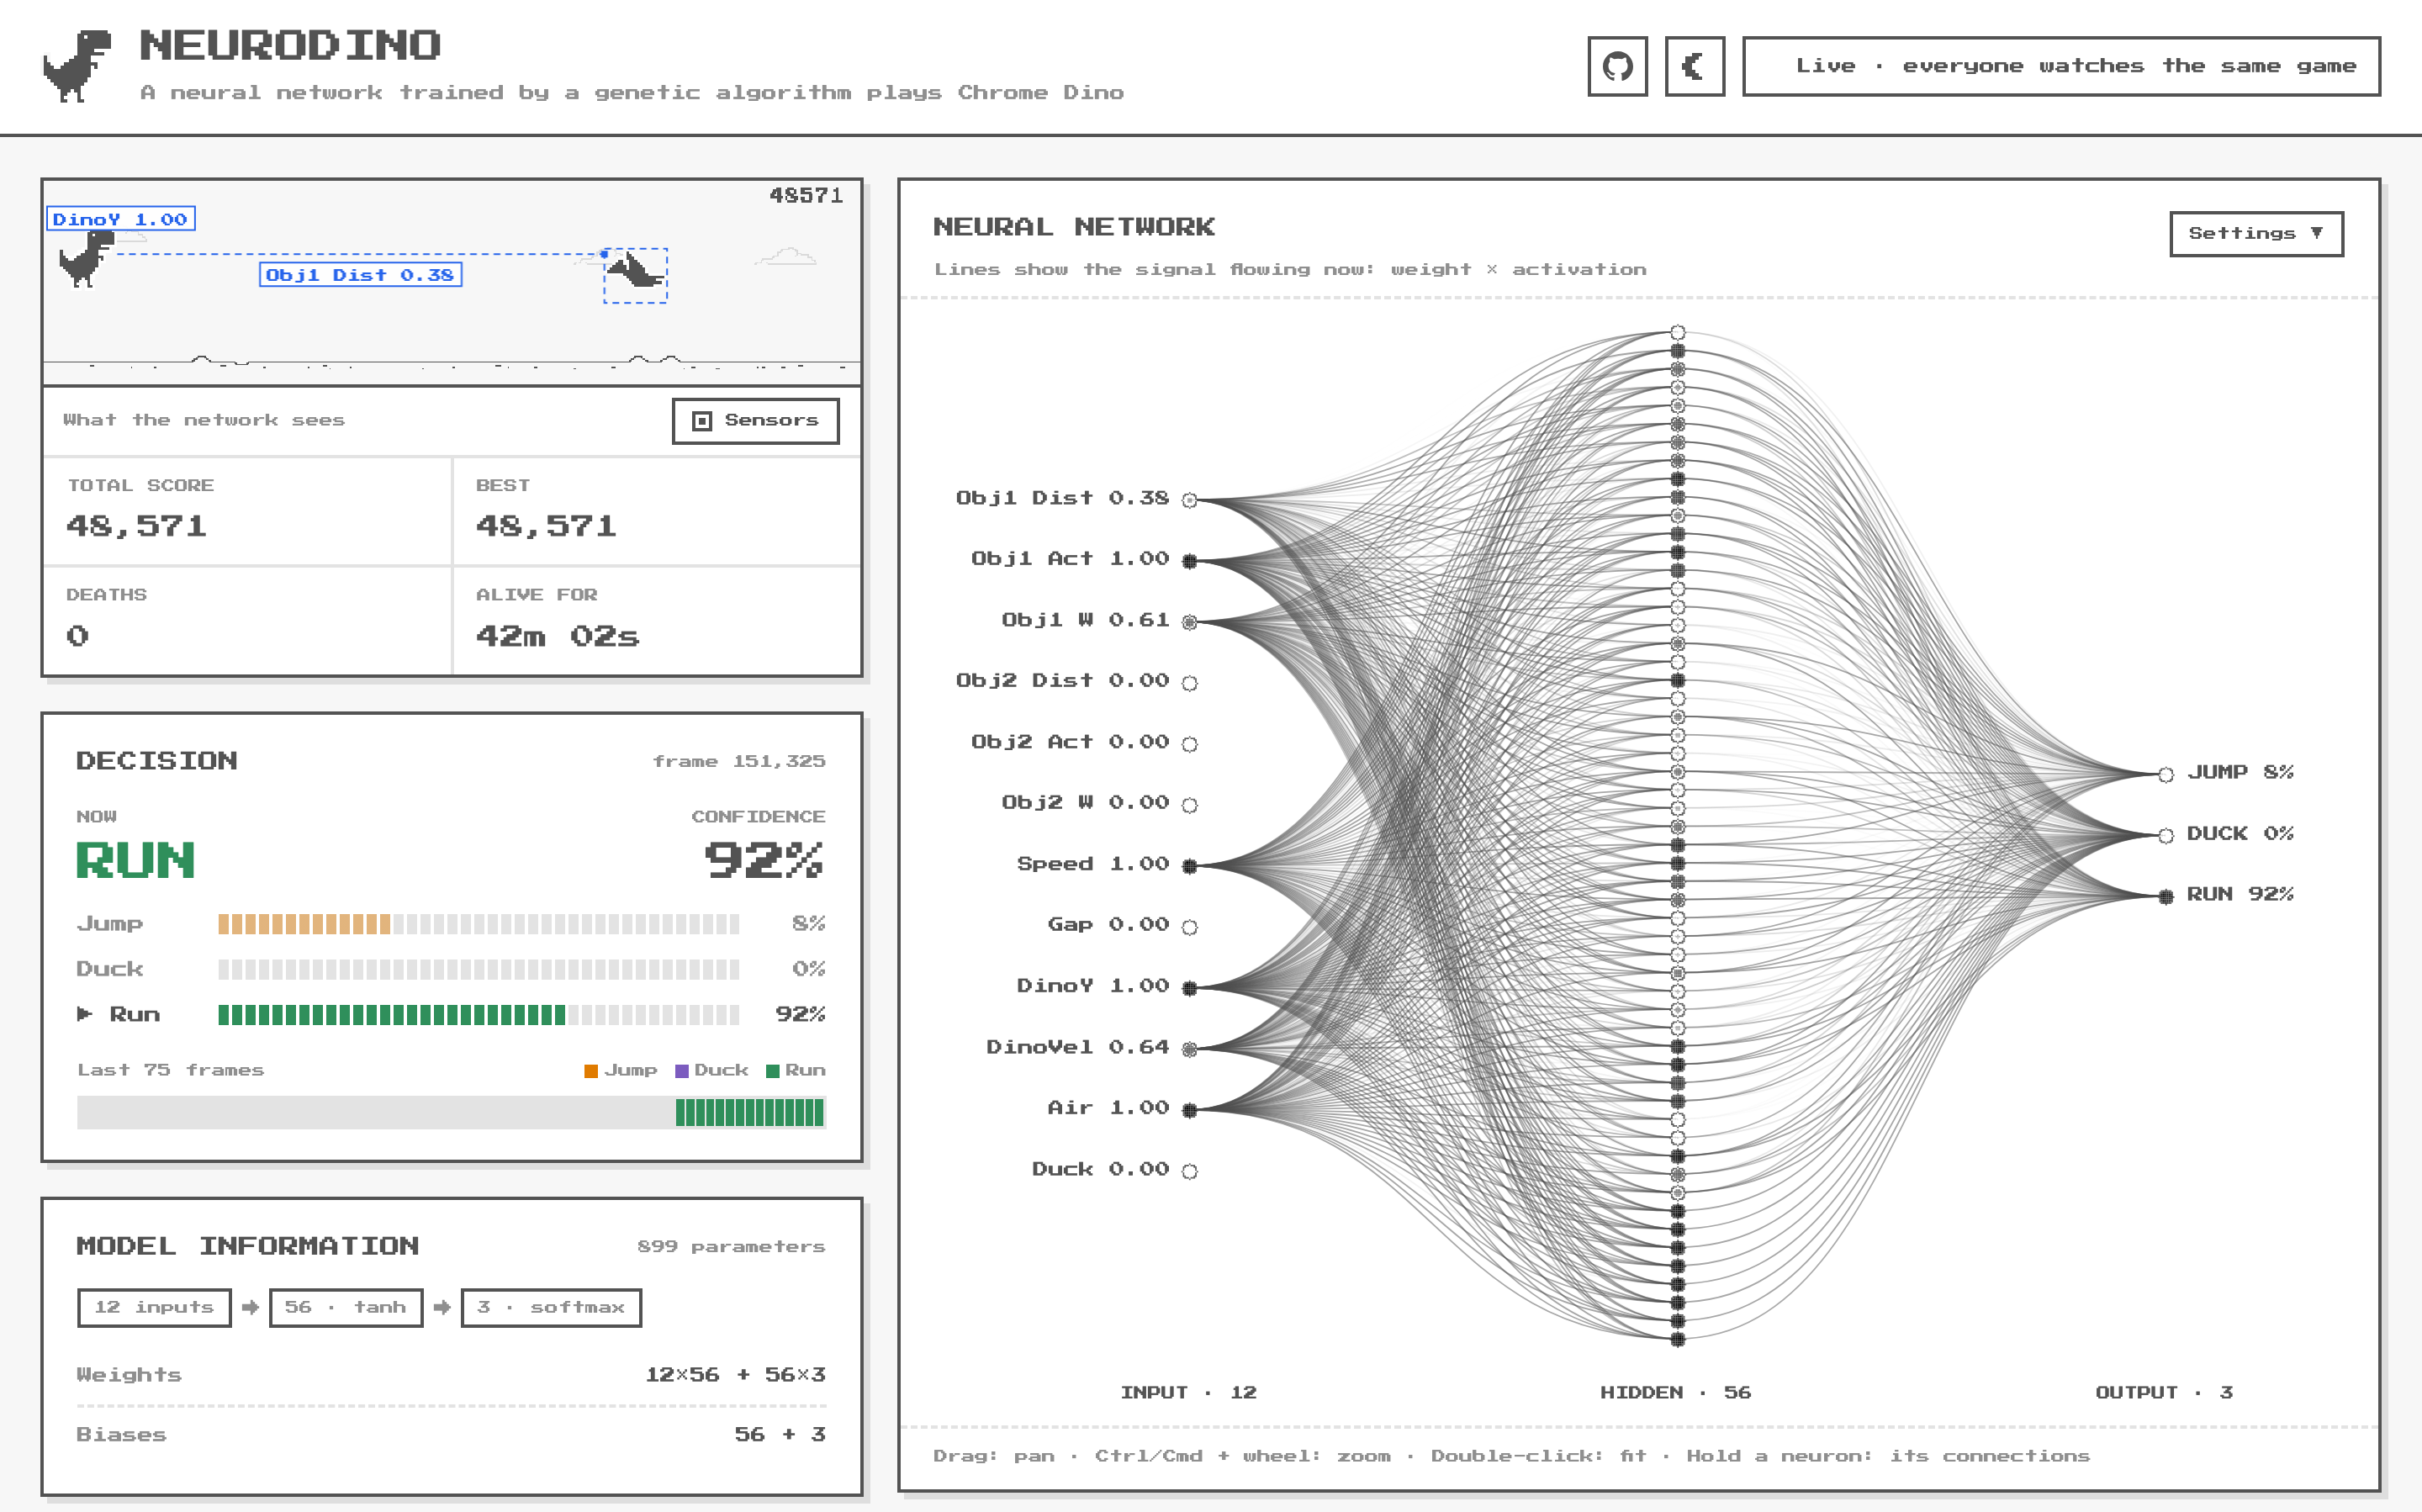
\includegraphics[width=\linewidth]{figures/website.png}
  \caption{Web sürümü. Solda oyun, sensörlerin ölçtüğü mesafeler ve ağın kararı, sağda ağ: her girdinin anlık değeri, gizli katman etkinlikleri ve üç eylemin olasılıkları. Site v3'ü oynatmaktadır (56 gizli nöron). Görüntüde dino havada, inişe geçmiştir; sıradaki engel, koşan dinonun üzerinden geçen en yüksek kuştur (Obj1 Act $= 1$).}
  \label{fig:site}
\end{figure}
\FloatBarrier

\subsection{Değerlendirme Protokolü}

Eğitilen ağ, web sürümündeki TypeScript oyun motoruyla yeni oyunlarda değerlendirilmiştir. 1'den 200'e kadar tohumlarla üç koşul oynatılmıştır:
\begin{itemize}
  \item \textbf{Eğitim koşulları:} eğitimdeki döngü sırası, normal boşluklar ve kapalı gece modu. Eğitimdeki sıra, ağa her karede bir önceki karenin sonundaki girdiler verilerek elde edilmiştir.
  \item \textbf{Web sitesi koşulları:} izleme döngüsü ve normal boşluklar; web sürümünün bugünkü hali.
  \item \textbf{Demo koşulları:} izleme döngüsü ve iki kat boşluklar; Gradio paneli ve izleme betiğinin varsayılan hali.
\end{itemize}
İlk iki koşulda her oyun dino ölene ya da 4 saatlik oyun süresi (864.000 kare) dolana kadar, üçüncüsünde en çok 30 dakika (108.000 kare) oynatılmıştır.

TypeScript motorunun sonuçları Python motoruyla doğrulanmıştır. Bunun için Python motoru aynı rastgele sayı akışını kullanacak biçimde çalıştırılmış ve web sürümünün zemin çizgisi için çektiği tek görsel rastgele sayı Python tarafında da çekilmiştir. Eğitim çalıştırıcısı (tek ajanla) 200 tohumun her birinde ilk 12.000 karede ve beş uzun oyunda (45.000 kareye kadar), izleme betiği ise iki boşluk modunda 400 oyunun her birinde ilk 20.000 karede ve iki uzun oyunda (230.000 kareye kadar) TypeScript motoruyla aynı karede aynı skorla ölmüş ya da aynı süre boyunca hayatta kalmıştır.

Her oyunda ölüm karesi, skoru ve hızı; öldüren engel (çarpışma anında dinoyla yatayda çakışan engel) ve o anda engelin sol kenarının dinonun sol kenarını geçip geçmediği; seçilen eylemler; her kuşun hangi eylemle geçildiği ve her girdinin dağılımı kaydedilmiştir. Maksimum hızdaki ölüm sıklığı, ölüm sayısının maksimum hızda geçen toplam oyun süresine bölünmesiyle hesaplanmış ve Poisson dağılımı için kesin \%95 güven aralığıyla verilmiştir \cite{garwood1936}. İki modelin ölüm sıklıkları, iki modeldeki toplam ölüm sayısına koşullu iki yönlü binom testiyle karşılaştırılmıştır.

Girdi ablasyonu eğitim koşullarında yapılmıştır: her girdi her karede (a) 0'a ya da (b) eğitim koşullarındaki değerlendirmede bütün karelerin ortalamasına sabitlenmiştir \cite{covert2021}. Her deney aynı 200 tohumla en çok 30 dakika oynatılmış ve maksimum hıza ulaşan ve 30 dakikayı tamamlayan oyunlar sayılmıştır. Değerlendirmenin ve doğrulamanın kodu ve verileri kod deposunda paylaşılmıştır.

\section{Bulgular}

\subsection{Eğitim Süreci}

Şekil~\ref{fig:training} her neslin en iyi ve ortalama skorunu, rekoru ve mutasyon oranını göstermektedir. İlk 41 nesilde en iyi skor 1.247'yi (30. nesil) geçmemiş ve bütün ajanlar hızlanma döneminde ölmüştür; 41. neslin bittiği anda hız 8,94'tü. 42. nesilde bir ajan hızlanma dönemini ilk kez atlatıp maksimum hıza ulaşmış ve en iyi skor 1.247'den 12.643'e çıkmıştır (yaklaşık 10 kat). 42. nesilden itibaren 42 neslin hepsinde en iyi ajan maksimum hıza ulaşmıştır. Rekor 43. nesilde 87.216'ya, 49. nesilde 109.871'e ve 77. nesilde 547.287'ye çıkmıştır; 77. nesil tek başına 63 dakika sürmüştür.

\begin{figure}[!htbp]
  \centering
  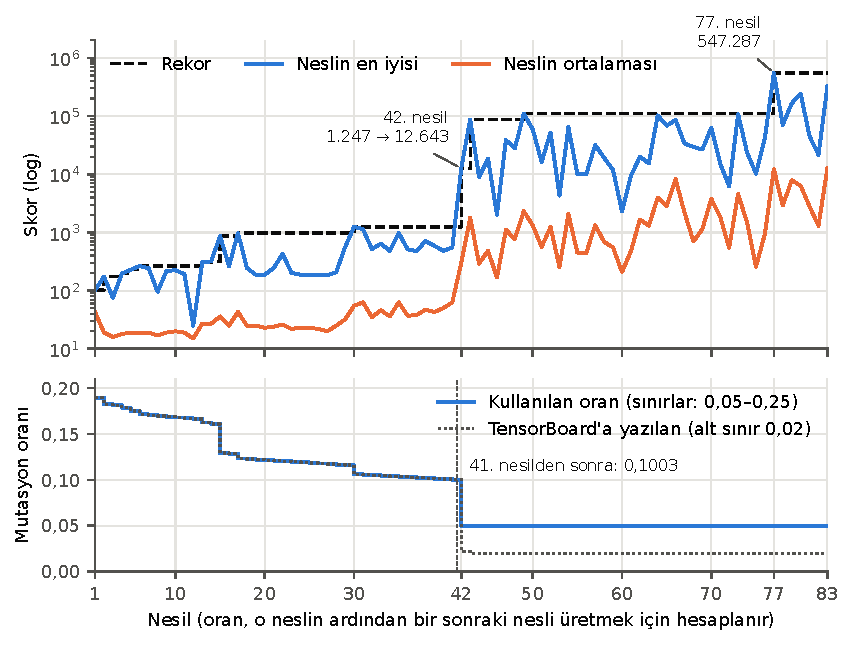
\includegraphics[width=\linewidth]{figures/training.pdf}
  \caption{Üstte her neslin en iyi ve ortalama skoru ile rekor (logaritmik ölçek), altta mutasyon oranı. Oran bir neslin ardından hesaplanır ve sonraki nesli üretir. Eğitimde kullanılan oran Denklem~\eqref{eq:rate} ile 0,05'te sınırlanır; TensorBoard'a yazılan değer ise 0,02 alt sınırıyla hesaplanmıştır.}
  \label{fig:training}
\end{figure}
\FloatBarrier

Mutasyon oranı ile skor sıçraması arasındaki ilişki sebep--sonuç yönünden dikkatle okunmalıdır. 42. nesli üreten oran, 41. nesilden sonra hesaplanan 0,1003'tür; yani sıçramadan önce oran 0,10'un altına düşmemiştir. Grafikteki keskin düşüş, 42. neslin rekorunun Denklem~\eqref{eq:rate}'e girmesiyle oluşur: formül 0,022 verir ve oran 0,05 alt sınırına iner. Düşüş sıçramanın sonucudur. Oran 42. nesilden sonra eğitimin sonuna kadar 0,05'te kalmıştır. Tek bir koşu ve bir kontrol deneyi (örneğin sabit oranlı bir koşu) olmadığı için sıçramanın uyarlamalı mutasyondan kaynaklandığı söylenemez.

Tek bölümlük uygunluk değerlendirmesi skorları şansa açık hale getirir. 547.287 puanlık ağ 78. nesle seçkin birey olarak değiştirilmeden aktarılmış, ancak 78. neslin en iyi skoru 70.721'de kalmıştır. Yani aynı ağ başka bir bölümde en fazla 70.721 puan yapmıştır; rekorun büyük bir kısmı o bölümün engel dizisine bağlıdır. Eğitim 83. nesilden sonra durdurulmuştur (83. neslin en iyi skoru 328.720).

\subsection{Ağırlıkların Dağılımı}

Şekil~\ref{fig:weights}, 1., 42. ve 77. nesillerde rekor kıran ağların ağırlık dağılımlarını göstermektedir. 1. nesildeki ağırlıklar Glorot başlatmasının tekdüze aralığındadır (giriş--gizli katman için $\pm 0{,}316$). Evrimle dağılımlar genişlemiştir: giriş--gizli ağırlıkların standart sapması 0,18'den 0,33'e ve 0,37'ye, gizli--çıkış ağırlıklarınınki 0,21'den 0,33'e ve 0,40'a çıkmıştır; 77. nesilde giriş--gizli ağırlıklar $-1{,}44$ ile $1{,}21$ arasındadır. Bu dağılımlar parametrelerin nasıl değiştiğini gösterir; tek başlarına ağın ne öğrendiğini açıklamaz. Çıkış katmanında yalnızca üç bias değeri olduğundan onların histogramı verilmemiştir.

\begin{figure}[!htbp]
  \centering
  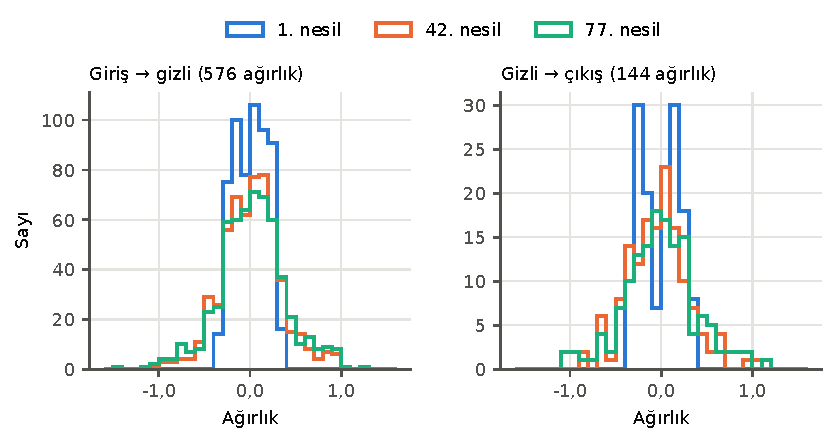
\includegraphics[width=\linewidth]{figures/weights.pdf}
  \caption{1., 42. ve 77. nesillerde rekor kıran ağların ağırlık dağılımları. Solda giriş--gizli, sağda gizli--çıkış katmanı.}
  \label{fig:weights}
\end{figure}
\FloatBarrier

\subsection{Değerlendirme}
\label{sec:eval}

Tablo~\ref{tab:conditions} ve Şekil~\ref{fig:eval} üç koşuldaki sonuçları özetlemektedir. Eğitim koşullarında ağ 200 oyunun 195'inde (\%97,5) maksimum hıza ulaşmıştır; erken biten beş oyunun hepsi 10,8 hızında, ${y = 75}$'teki kuşla bitmiştir. Maksimum hızda ise ölümler zamanla birikmektedir: oyunların 180'i 30 dakikayı, 151'i 2 saati, 110'u (\%55) 4 saati (280.208 puan) tamamlamıştır. Maksimum hızda oynanan toplam yaklaşık 600 saatte 85 ölüm, yani saatte yaklaşık 0,14 ölüm (\%95 güven aralığı 0,11--0,18) görülmüştür. Bu, eğitimdeki skorlarla tutarlıdır: 547.287 puanlık rekor bölümü yaklaşık 7,8 saat, aynı ağın 78. nesildeki bölümü ise en fazla yaklaşık 1 saat (70.721 puan) sürmüştür.

\begin{table}[!htbp]
  \centering
  \small
  \caption{200 yeni oyunda maksimum hıza ulaşan, 30 dakikayı ve 4 saati tamamlayan oyun sayıları. Demo koşullarında oyunlar en çok 30 dakika oynatılmıştır.}
  \label{tab:conditions}
  \begin{tabular}{@{}l l l r r r@{}}
    \toprule
    Koşul & Döngü & Boşluklar & Maks. hız & 30 dakika & 4 saat \\
    \midrule
    Eğitim & Eğitimdeki & Normal & 195 & 180 & 110 \\
    Web sitesi & İzleme & Normal & 87 & 86 & 85 \\
    Demo & İzleme & İki kat & 110 & 110 & -- \\
    \bottomrule
  \end{tabular}
\end{table}
\FloatBarrier

Web sitesi koşullarında tablo tersine döner. Oyunların 113'ü (\%56,5) maksimum hıza ulaşmadan bitmiştir; bu ölümler dört dar hız aralığında toplanmıştır (yaklaşık 7,0; 9,7--10,0; 10,5--10,8 ve 12,7--12,8). Maksimum hıza ulaşan 87 oyunun ise yalnızca ikisi 4 saat içinde ölmüştür (23.154 ve 74.243 puanda). Demo koşullarında boşluklar büyüdüğü için 7 civarındaki kaktüs ölümleri ortadan kalkmış, oyunların 90'ı (\%45) erken bitmiş, maksimum hıza ulaşan 110 oyunun hiçbiri 30 dakika içinde ölmemiştir.

\begin{figure}[!htbp]
  \centering
  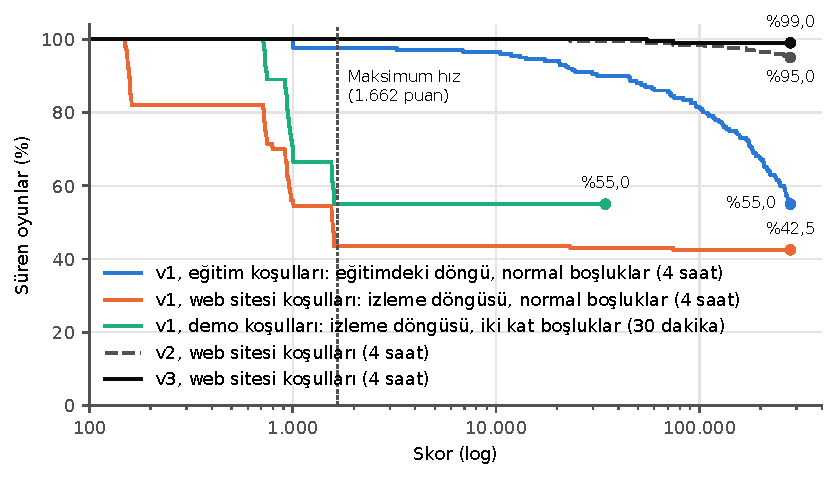
\includegraphics[width=\linewidth]{figures/evaluation.pdf}
  \caption{200 yeni oyundan belirli bir skora ulaşanların oranı: v1 üç koşulda, v2 ve v3 web sitesi koşullarında (yatay eksen logaritmik). Dikey kesikli çizgi maksimum hıza ulaşılan skoru gösterir. Eğitim ve web sitesi koşullarında oyunlar 4 saate, demo koşullarında 30 dakikaya kadar oynatılmıştır. Gri kesikli eğri Bölüm~\ref{sec:v2}'teki ikinci eğitimle elde edilen v2, siyah eğri Bölüm~\ref{sec:v3}'daki v3'tür.}
  \label{fig:eval}
\end{figure}
\FloatBarrier

\subsection{Davranış Analizi}

\textbf{Ağ hiç eğilmemektedir.} Eğitim koşullarındaki 131,1 milyon karenin hiçbirinde \emph{eğil} eylemi seçilmemiştir. ${y = 75}$'teki 290.857 kuşun biri dışında hepsinin, ${y = 100}$'deki 290.178 kuşun üçü dışında hepsinin üzerinden zıplanmıştır. Bu, girdi tasarımının doğrudan bir sonucudur: Act girdisi ${y = 75}$ ve ${y = 100}$'deki kuşlar için aynı değeri verir ve bu iki kuşu birlikte geçmenin tek yolu zıplamaktır. Eğilmek ${y = 75}$'teki kuş için işe yarar, ${y = 100}$'deki kuş için ölümcüldür.

\textbf{Ölümler zıplama zamanlamasından kaynaklanmaktadır.} Ölüm anındaki geometri iki türü ayırır. Engelin sol kenarı dinonun sol kenarını geçmişse dino engelin üzerine inmiştir, yani erken zıplamıştır; engel hâlâ dinonun önündeyse dino geç zıplamış ya da hiç zıplamamıştır. Eğitim koşullarında maksimum hızdaki 85 ölümün hepsi ikinci türdendir (72'si büyük kaktüs, 13'ü ${y = 75}$'teki kuş); erken biten beş oyun ise birinci türdendir. Web sitesi koşullarında 113 erken ölümün hepsi birinci türdendir. İzleme döngüsünde ağ engeli bir kare daha yakında gördüğü için zıplama kararı bir kare erken tetiklenir; bu, ara hızlarda engelin üzerine inmeye yol açarken maksimum hızdaki geç zıplamaları büyük ölçüde ortadan kaldırır (web sitesi koşullarında maksimum hızdaki iki ölüm de ikinci türdendir; bu tür ölümlerin nedeni Bölüm~\ref{sec:v3}'da incelenmiştir).

\textbf{Ağ girdilerin yalnızca bir kısmını kullanmaktadır.} Tablo~\ref{tab:ablation} her girdinin eğitim koşullarında ne sıklıkla sıfırdan farklı olduğunu ve ablasyonun sonuçlarını vermektedir. Gap girdisi 131,1 milyon karenin hiçbirinde 0'dan farklı olmamıştır: normal boşluklarla iki engel arasındaki süre hiçbir zaman 15 karenin altına düşmez. Duck girdisi de ağ hiç eğilmediği için hep 0'dır. İkinci engelin girdileri karelerin yalnızca yaklaşık \%5'inde sıfırdan farklıdır.

\begin{table}[!htbp]
  \centering
  \small
  \caption{Eğitim koşullarında girdi kullanımı ve ablasyon. Sıfırdan farklı: 200 oyunun bütün karelerinde girdinin 0'dan farklı olduğu karelerin oranı. Ablasyon sütunları, 200 oyundan maksimum hıza ulaşan / 30 dakikayı tamamlayan oyun sayısıdır; ablasyonsuz değerlendirmede bu sayılar 195 / 180'dir. * işaretli deneylerde 200 oyunun her birinin sonucu (ölüm karesi ve skoru) ablasyonsuz değerlendirmeyle birebir aynıdır.}
  \label{tab:ablation}
  \begin{tabular}{@{}l r c r c@{}}
    \toprule
    Girdi & Sıfırdan farklı & 0'a sabit & Ortalama & Ortalamaya sabit \\
    \midrule
    Obj1 Dist & \%92,5 & 0 / 0 & 0,494 & 0 / 0 \\
    Obj1 Act & \%10,7 & 0 / 0 & 0,107 & 0 / 0 \\
    Obj1 W & \%92,6 & 0 / 0 & 0,536 & 171 / 116 \\
    Obj2 Dist & \%4,8 & 195 / 180* & 0,008 & 183 / 169 \\
    Obj2 Act & \%0,6 & 194 / 179 & 0,006 & 197 / 181 \\
    Obj2 W & \%4,9 & 156 / 142 & 0,029 & 140 / 129 \\
    Speed & \%100 & 0 / 0 & 0,997 & 0 / 0 \\
    Gap & \%0 & 195 / 180* & 0 & 195 / 180* \\
    DinoY & \%58,6 & 195 / 180* & 0,537 & 0 / 0 \\
    DinoVel & \%58,6 & 195 / 180* & 0,037 & 107 / 66 \\
    Air & \%58,6 & 195 / 180* & 0,586 & 0 / 0 \\
    Duck & \%0 & 195 / 180* & 0 & 195 / 180* \\
    \bottomrule
  \end{tabular}
\end{table}
\FloatBarrier

0'a sabitleme, girdinin taşıdığı bilginin kaldırılmasına karşılık gelir. Altı girdi (Obj2 Dist, Gap, DinoY, DinoVel, Air ve Duck) sıfırlandığında 200 oyunun hiçbirinin sonucu değişmemiş, Obj2 Act'in sıfırlanması sonuçları çok az değiştirmiştir. Havadayken anlam taşıyan DinoY, DinoVel ve Air'in etkisizliği beklenen bir sonuçtur: dino havadayken ağın kararı ancak hızlı düşüş (\emph{eğil}) seçilirse bir şey değiştirir ve ağ bu eylemi hiç seçmez; dino yerdeyken ise bu girdiler zaten 0'dır. Buna karşılık en yakın engelin mesafesi, Act girdisi, genişliği ya da oyun hızı sıfırlandığında ajan hiçbir oyunda maksimum hıza ulaşamamıştır. Act'in rolü eğilmek değildir: Act sıfırlandığında 200 ölümün 199'u ${y = 50}$'deki kuşa çarpmaktan olmuştur; ağ bu girdiyi, en yüksek kuş yaklaşırken zıplamasını ona çarpmayacak biçimde ayarlamak için kullanmaktadır. Obj2 W'nin sıfırlanması ise sonucu kötüleştirmiştir (195 yerine 156 oyun maksimum hıza ulaşmıştır).

Ortalamaya sabitleme ise örneğin yerdeyken 0 olan girdileri sıfırdan farklı yaptığı için ağı eğitimde görmediği girdi birleşimlerine sokar; bu sütun girdinin bilgisinden çok ağın küçük kaymalara duyarlılığını ölçer. İki sonuç zamanlama bulgusunu doğrudan desteklemektedir. Speed'in ortalamasına (0,997, yani neredeyse maksimum hız) sabitlenmesiyle 200 oyunun hepsi hızlanma döneminde bitmiş ve hepsinde dino engelin üzerine inmiştir: ağ her hızda maksimum hızdaymış gibi erken zıplamıştır, yani zıplama anını oyun hızına göre ayarlamaktadır. DinoVel'in ortalamasına (0,037) sabitlenmesi ise dino yerdeyken normalde 0 olan bu girdiye küçük bir kayma ekleyerek zıplamayı geciktirmiştir: 30 dakika içinde biten oyun sayısı 20'den 134'e çıkmış ve bu ölümlerin hiçbirinde dino engelin üzerine inmemiştir. Benzer bir kayma (0,036) web sitesi koşullarında ise izleme döngüsünün bir kare erken kararını dengelemiş ve 200 oyunun hepsinin maksimum hıza ulaşmasını sağlamıştır.

\section{İkinci Eğitim (v2)}
\label{sec:v2}

Bulgular iki soruna işaret ediyordu: eğitim ile demonun döngü sırası farklıydı ve tek bölümlük uygunluk farklı oyunlara karşı sağlamlığı ödüllendirmiyordu. Bu nedenle eğitim kodu değiştirilerek v1'den başlayan ikinci bir koşu yapılmıştır.

\textbf{Yöntem.} Eğitim, web sürümünün döngüsünü (önce engeller ilerler, sonra ağ karar verir) ve gece modunu içeren yeni bir oyun modülüyle yapılmıştır. Bu modülün, aynı rastgele sayı akışıyla web sürümünün oyunlarını birebir ürettiği 200 tohumda doğrulanmıştır. Engeller ajanların eylemlerinden bağımsız olduğu için bir oyundaki her ajan, tek başına oynasaydı oynayacağı oyunun aynısını oynar. Her nesilde 50 ağ aynı 10 oyunu oynar; oyunlar her nesilde yenilenir, en çok 60 dakika sürer ve 10 işlemci çekirdeğinde paralel oynatılır. Bir ağın uygunluğu 10 oyundaki ortalama skorudur. Seçkincilik, seçilim ve çaprazlama v1'deki gibidir; mutasyon oranının alt sınırı 0,02'ye indirilmiş ve şok mutasyonu kaldırılmıştır. İlk popülasyon v1 ve onun 0,05 oranında mutasyona uğratılmış 49 kopyasıdır. Bütün tohumlar sabittir; koşu aynen tekrarlanabilir.

Bu ayarlara bir ön denemeden sonra varılmıştır. Oyunların 30 dakikada kesildiği ve v1'in mutasyon ayarlarının kullanıldığı ilk denemede bulunan en iyi ağ erken ölümleri kaldırmış, ancak maksimum hızda oyunların \%9'unda 30 dakika içinde ölmüştür: 30 dakikalık oyunlar maksimum hızdaki sağlamlığı uygunluğa yeterince yansıtmıyordu. Ayrıca popülasyonun medyan skoru yaklaşık 50--300 puanda kalıyor, yani çocukların çoğu ilk engellerde ölüyordu; şok mutasyonu kaldırıldığında ilk neslin medyan skoru 308'den 4.090'a çıkmıştır.

\textbf{Model seçimi.} 40 nesil, Apple M4 üzerinde 56,8 dakika sürmüştür. Her neslin en iyisi, eğitimde kullanılmayan 100 doğrulama oyununda 30 dakika boyunca değerlendirilmiştir. 3. nesilde bulunan ağ doğrulamada en iyisidir (ortalama 34.008 puan, oyunların \%97'si tamamlandı; v1: 15.288 puan, \%43) ve seçkin birey olarak 40. nesle kadar her neslin en iyisi kalmıştır. Bu ağ, 1001--1100 tohumlarıyla 100 oyunda 4 saat boyunca da oynatılmış; hiç erken ölmemiş, maksimum hızda 392 saatte 3 kez ölmüştür. v2 olarak bu ağ seçilmiştir. Test tohumları (1--200) seçim bitene kadar kullanılmamıştır.

\begin{table}[!htbp]
  \centering
  \small
  \caption{v1 ve v2, web sitesi ve demo koşullarında 200 test oyununda.}
  \label{tab:v2}
  \begin{tabular}{@{}l l r r r@{}}
    \toprule
    Model & Koşul & Maks. hız & 30 dakika & 4 saat \\
    \midrule
    v1 & Web sitesi & 87 & 86 & 85 \\
    v2 & Web sitesi & 200 & 199 & 190 \\
    v1 & Demo & 110 & 110 & -- \\
    v2 & Demo & 200 & 200 & -- \\
    \bottomrule
  \end{tabular}
\end{table}
\FloatBarrier

\textbf{Sonuçlar.} Tablo~\ref{tab:v2} ve Şekil~\ref{fig:eval}'teki gri kesikli eğri v2'nin test sonuçlarını göstermektedir. v2 web sitesi koşullarında 200 oyunun hepsinde maksimum hıza ulaşmış ve 190'ında 4 saati tamamlamıştır; v1 aynı oyunların 113'ünde hızlanma döneminde ölmüştü. Maksimum hızda 775 saatte 10 ölüm, yani yaklaşık 78 saatte bir ölüm (\%95 güven aralığı 42--162 saatte bir) görülmüştür; bu ölümlerin hepsi ikinci türdendir ve nedenleri Bölüm~\ref{sec:v3}'da incelenmiştir. Demo koşullarında da 200 oyunun hepsi 30 dakikayı tamamlamıştır. Sonuçlar Python motoruyla da kontrol edilmiştir: 200 tohumun ilk 8.000 karesinde hiç erken ölüm olmamış, üç uzun oyundaki ölümler aynı karede ve aynı skorla gerçekleşmiştir. Act girdisi değişmediği için v2 de hiç eğilmemektedir: 168,8 milyon karenin hiçbirinde \emph{eğil} seçilmemiştir.

\section{Üçüncü Model (v3): Havada Hızlı Düşüş}
\label{sec:v3}

\textbf{Sorun.} v2, maksimum hızda ortalama yaklaşık 100 saatte bir ölmektedir. Test oyunlarındaki 10 ölümün hepsi aynı durumda gerçekleşmiştir: tek bir küçük kaktüsün ardından 321--381 piksel (yaklaşık 25--29 kare) içinde ikinci bir engel gelir. Maksimum hızda bir zıplama 33 kare sürer ve dinoyu yaklaşık 430 piksel taşır; dino ikinci engel için zıplaması gereken anda hâlâ havadadır. Bu ölümlerin her biri, ölümden 60 kare önceki durumdan yeniden oynatılmış ve bu 60 karenin her birinde tek bir değişiklik denenmiştir: o kareden başlayarak birkaç kare eğilmek (havadayken hızlı düşüş), o karede zıplamak ya da zıplamayı birkaç kare geciktirmek. Eğilmek 10 ölümün 10'unu önlemiş, daha erken ya da daha geç zıplamak hiçbirini önlememiştir. v2 bu eylemi hiç kullanmaz.

\textbf{Genetik algoritmayla deneme.} Önce v2'den başlayan ve ağları bu zor anlarda hayatta kalmalarına göre puanlayan bir genetik algoritma denenmiştir. Ölümlere giden karelerde dino havadayken v2'nin \emph{eğil} çıkışı (softmax öncesi), en yüksek çıkışın en az 1,45 (medyan 2,8) altındadır. Küçük mutasyonlar onu neredeyse hiç öne geçirmediği için ağların puanları değişmemiş ve seçilim ilerleyememiştir.

\textbf{Yöntem.} v2 4.000 oyunda (100001--104000 tohumları, 4'er saat) oynatılmış ve maksimum hızdaki 156 ölümünün her birinden 45, 60, 90 ve 120 kare önceki oyun durumları kaydedilmiştir. Etiketler, motorda iki seçeneğin de gerçekten oynatılmasıyla elde edilmiştir. Havadaki bir kareden oyun iki kez 150 kare oynatılır: birinde dino o karede eğilir, diğerinde eğilmez; iki oyunda da dino yere inene kadar başka eğilme yoktur, sonrasında v2 oynar. Yalnızca eğilen oyun hayatta kalıyorsa kare ``eğilmeli'', yalnızca eğilmeyen kalıyorsa ``eğilmemeli'' olarak etiketlenir; ikisi de kalıyorsa gereksiz her eğilme yeni bir risk olduğundan ``eğilmemeli'' sayılır. Bu yolla 100 normal oyunun (600001--600100) her beşinci hava karesi ve ölüm anlarından sonraki bütün hava kareleri etiketlenmiştir; her beşinci ölüm oyununun anları değerlendirme için ayrılmıştır. Sonuçta 4.909 ``eğilmeli'' ve 1.302.056 ``eğilmemeli'' hava karesi ile 200 normal oyundan (500001--500200) 2.260.900 yer karesi elde edilmiştir.

v3, v2'ye yalnızca \emph{eğil} çıkışına bağlanan 8 gizli nöron eklenerek oluşturulmuştur (12--56--3, 899 parametre). Yeni nöronlar ve eğil satırı, bu etiketlerle Adam \cite{kingma2015} kullanılarak gradyan inişiyle eğitilmiştir (20.000 adım, 16.384'lük yığınlar). Yer karelerinde hedef v2'nin kararıdır. v2'nin 48 nöronu ile zıpla ve koş satırları dondurulmuştur; v2 hiç eğilmediğinden v3, eğilmediği her karede v2 ile aynı kararı verir. Eğitimden sonra eğil çıkışının bias'ı 1 azaltılmıştır. Bu değer, kaydedilen anlarda kurtaran eğilmeleri koruyup gereksiz olanları azalttığı için seçilmiştir: 1 azaltılmış ağ, eğitimde kullanılmayan 124 ölüm anının 103'ünü kurtarır (azaltmadan önce 74, 2 azaltınca 77) ve dinonun normalde geçtiği 4.000 dar anın hepsini geçer.

\textbf{Süre ve tekrarlanabilirlik.} v2'den v3'e giden zincir, 10 çekirdekli bir Apple M4 üzerinde 10 paralel süreçle yaklaşık 37 dakika sürmektedir: ölüm anlarının toplanması 31 dakika, normal oyunlardan örnek alınması ve etiketleme 3,4 dakika, gradyan inişi 2,3 dakika. Bir adayın 1.000 dört saatlik doğrulama oyununda değerlendirilmesi 8,4 dakika daha sürer. Bütün tohumlar sabit olduğundan zincir yeniden çalıştırıldığında aynı veriyi ve bit düzeyinde aynı v3'ü üretmiştir.

\textbf{İşe yaramayanlar.} Kaydedilen anlardaki başarı uzun oyundaki başarıyı göstermemiştir; adaylar 300001--301000 tohumlarıyla 1.000 dört saatlik doğrulama oyununda karşılaştırılmıştır. Aynı oyunlarda v2 30 kez ölmüştür. Ağın tamamının eğitilmesi (646 ölüm), ağa iniş süresini veren iki yeni girdi eklenmesi (551) ve bias azaltılmadan eklenen nöronlar (125), etiketlere iyi uymalarına karşın ölümleri artırmıştır: başka yerlerde değişen birkaç karar, kurtardıklarından çok daha fazlasına mal olmuştur. Yalnızca eğil satırının eğitilmesi ise az fark yaratmıştır (23). Eklenen nöronlarla birlikte bias 1 azaltıldığında ölüm sayısı 6'ya inmiş, 2 azaltıldığında 9 olmuştur.

\begin{table}[!htbp]
  \centering
  \small
  \caption{v2 ve v3, web sitesi koşullarında dört saatlik oyunlarda. Yeni oyunlar (900001--901000) hiçbir modelin daha önce oynamadığı oyunlardır.}
  \label{tab:v3}
  \begin{tabular}{@{}l l r r r r@{}}
    \toprule
    Model & Oyunlar & Maks. hız & 4 saat & Maks. hızda ölüm & Maks. hızda saat \\
    \midrule
    v2 & 200 test & 200 & 190 & 10 & 775 \\
    v3 & 200 test & 200 & 198 & 2 & 787 \\
    v2 & 1.000 yeni & 1.000 & 960 & 40 & 3.893 \\
    v3 & 1.000 yeni & 1.000 & 997 & 3 & 3.961 \\
    \bottomrule
  \end{tabular}
\end{table}
\FloatBarrier

\textbf{Sonuçlar.} v3 doğrulama oyunlarına bakılarak seçildiği için hiçbir modelin oynamadığı 1.000 yeni oyunda da v2 ile karşılaştırılmıştır (Tablo~\ref{tab:v3}). v2 bu oyunlarda 40 kez, yani yaklaşık 100 saatte bir (\%95 güven aralığı 71--136 saatte bir), v3 ise 3 kez, yani yaklaşık 1.300 saatte bir (\%95 güven aralığı 450--6.400 saatte bir) ölmüştür. Üç ölüm, v3'ün ölüm sıklığını ancak geniş bir aralıkla belirler: v3 v2'den yaklaşık 14 kat daha seyrek ölmektedir ve bu oranın \%95 güven aralığı 4--69 kattır. Fark rastlantıyla açıklanamaz: iki modelin ölüm sıklığı aynı olsaydı, 43 ölümün en fazla 3'ünün v3'e düşme olasılığı çok küçük olurdu (iki yönlü binom testi, $p \approx 10^{-9}$). Test oyunlarında v3 200 oyunun 198'inde 4 saati tamamlamıştır (Şekil~\ref{fig:eval}, siyah eğri); iki ölümü, v2'nin de öldüğü iki oyundadır. v3 bu oyunları seçimden önce hiç oynamamıştır, ancak sorunun tanısı v2'nin bu oyunlardaki ölümlerine bakılarak konduğu için test oyunları v3 açısından tamamen bağımsız sayılmamalıdır; bağımsız karşılaştırma yeni oyunlardır. Erken ölüm her iki modelde de yoktur. v3 1.000 yeni oyunda toplam 1.418 karede, yani nadiren eğilmiştir. Sonuçlar Python motoruyla da kontrol edilmiştir: 200 tohumun ilk 20.000 karesi ve iki uzun oyundaki ölümler aynıdır.

\section{Tartışma ve Sınırlılıklar}

Bulgular, küçük bir ağın öğrendiği politikanın oyun döngüsündeki tek karelik bir farka ne kadar duyarlı olabileceğini göstermektedir. Ağ eğitimde kararını engellerin bir kare önceki konumlarına göre vermeyi öğrenmiştir; izleme döngüsünde aynı ağ sistematik olarak bir kare erken zıplar. Bu nedenle demoda ve web sitesinde gözlenen davranış eğitim koşullarındaki davranışı temsil etmez. Maksimum hıza ulaşan koşuların izleme döngüsünde çok uzun sürmesi ağın genel bir özelliği değildir: aynı normal boşluklarla, izleme döngüsünde maksimum hıza ulaşan 87 oyunun yalnızca ikisi 4 saat içinde ölürken eğitimdeki döngüde 195 oyunun 85'i ölmüştür. Bir modelin eğitildiği ortamdan küçük bir farkla ayrılan bir ortamda değerlendirilmesinin sonuçları ne kadar değiştirebileceğine dair açık bir örnektir.

Tek bölümlük uygunluk değerlendirmesi de sonuçları etkiler. Bir nesildeki 50 ajan aynı tek bölümü oynadığı için skorlar o bölümün engel dizisine ve şansa bağlıdır; rekor kıran ağın bir sonraki nesilde en fazla 70.721 puan yapması bunu göstermektedir. Maksimum hızda saatte yaklaşık 0,14 ölümle 7,8 saatlik bir bölüm de şanslı bir bölümdür. v2'de her bireyin 10 farklı oyunda değerlendirilmesi ve eğitimin web sürümünün döngüsünde yapılması, yalnızca 40 nesilde hem erken ölümleri kaldırmış hem de maksimum hızdaki sağlamlığı korumuştur.

v3, seyrek bir hatanın düzeltilmesinin zorluğunu da göstermektedir. Hızlı düşüş yaklaşık 100 saatte bir gerekirken yanlış bir düşüş için her saniye fırsat vardır; bu yüzden düzeltme neredeyse hiç yanılmamalıdır. Kaydedilen zor anlarda iyi görünen birçok aday uzun oyunda v2'den kötü çıkmıştır. Sonuç veren yol, v2'nin kararlarını tamamen koruyup eklenen nöronlara yalnızca ``ne zaman düşmeli'' sorusunu öğretmek ve adayları uzun oyunlarla değerlendirmek olmuştur.

Çalışmanın başlıca sınırlılıkları şunlardır:
\begin{itemize}
  \item v1 tek bir koşudan oluşur ve sabit bir rastgelelik tohumu kullanılmamıştır; v2 sabit tohumlarla tekrarlanabilir, ancak o da tek bir koşudur. Kontrol deneyi olmadığı için uyarlamalı mutasyonun ya da diğer hiperparametrelerin etkisi hakkında bir sonuç çıkarılamaz.
  \item v3 yalnızca nöroevrimle eğitilmemiştir: eklenen nöronlar, motordaki aramayla etiketlenmiş karelerden gradyan inişiyle öğrenmiştir. Eğil bias'ındaki azaltım ve aday seçimi de elle yapılmıştır.
  \item v3'ün ölüm sıklığı yalnızca 3 ölüme dayandığından geniş bir belirsizlikle bilinmektedir (450 ile 6.400 saatte bir); daha dar bir aralık için çok daha uzun bir değerlendirme gerekir.
  \item Ajan başka yöntemlerle (NEAT, derin pekiştirmeli öğrenme ya da kural tabanlı bir ajan) karşılaştırılmamıştır.
  \item Girdi tasarımının üç kusuru vardır: Act eşiği eğilmeyi gerektiren kuşu işaretlemez (v3 de yalnızca havada hızlı düşmek için eğilir, kuşların altından geçmeyi bilmez), Gap girdisi normal boşluklarla hiçbir zaman 0'dan farklı olmaz ve DinoY havada geçen sürenin yaklaşık \%85'inde 1'de doyar.
  \item Ajan en fazla iki engeli görür ve mesafe girdileri en fazla 50 kare ilerisini ayırt eder; hız 6'dayken bu yaklaşık 300 piksel, yani ekranın yarısıdır.
  \item Değerlendirmenin tamamı TypeScript motoruyla yapılmıştır. Motorun Python motoruyla aynı sonucu verdiği, model ve döngüye göre her tohumun ilk 8.000 ile 20.000 karesinde ve on iki uzun oyunda doğrulanmış, ancak 4 saatlik oyunların tamamı Python'da tekrarlanmamıştır.
\end{itemize}

Gelecek çalışmalarda Act girdisinin kuşun üç yüksekliğini ayırt edecek biçimde yeniden tasarlanması ve ajanın kuşların altından eğilmeyi de öğrenmesi, birden çok tohumla tekrarlanan koşular ve başka yöntemlerle karşılaştırma planlanmaktadır.

\section{Sonuçlar}

Chrome T-Rex oyunu için Python ve Pygame tabanlı bir eğitim ortamı kurulmuş ve 771 parametreli sabit topolojili bir ağ genetik algoritmayla 6,55 saatte 83 nesil eğitilmiştir. Eğitimdeki belirgin sıçrama, 42. nesilde bir ajanın hızlanma dönemini ilk kez atlatmasıyla gerçekleşmiştir; mutasyon oranındaki düşüş bu sıçramanın sonucudur. Eğitim koşullarında rekortmen ağ 200 yeni oyunun \%97,5'inde maksimum hıza ulaşmış, maksimum hızda saatte yaklaşık 0,14 ölümle oyunların \%55'inde 4 saati tamamlamıştır. Web sitesinin ve demonun döngüsünde ağ her kararı bir kare daha güncel bilgiyle verdiği için sonuçlar tersine döner: oyunların \%56,5'i hızlanma döneminde biter, maksimum hıza ulaşanlar ise neredeyse hiç ölmez. Ağ hiç eğilmemekte, kararlarını fiilen en yakın engelin mesafesi, türü ve genişliği ile oyun hızına dayandırmakta ve başarısı zıplamanın yaklaşık bir karelik zamanlamasına bağlı kalmaktadır. Eğitimin web sürümünün döngüsünde ve her bireyin 10 oyunda değerlendirildiği bir düzenle tekrarlanması bu sorunu 40 nesilde gidermiştir: v2, 200 test oyununun hepsinde maksimum hıza ulaşmış ve 190'ında 4 saati tamamlamıştır. v2'nin kalan ölümleri, dinonun bir engeli zıpladıktan sonra sonraki engel için vaktinde yere inememesinden kaynaklanmaktadır; havada hızlı düşmeyi öğrenen 8 ek nöronla elde edilen v3, hiçbir modelin oynamadığı 1.000 dört saatlik oyunda ölümleri 40'tan 3'e, yani yaklaşık 14 kat (\%95 güven aralığı 4--69 kat) azaltmıştır. Herkesin aynı oyunu aynı anda izlediği deterministik web sürümü artık v3'ü oynatmakta ve ağın kararlarını canlı olarak gözlemlemeyi sağlamaktadır.

\section*{Kod ve Veri}

Eğitim ve oyun kodu, üç model, eğitim kayıtları, v3'ün eğitim betikleri (\texttt{training/}) ve değerlendirme betikleri ile oynatılan bütün oyunlar (\texttt{evaluation/}) \url{https://github.com/ahm3texe/NeuroDino} adresindedir. Model \url{https://huggingface.co/ahm3texe/neurodino}, canlı web sürümü \url{https://huggingface.co/spaces/ahm3texe/neurodino} adresinde yayındadır.

\begin{thebibliography}{99}

\bibitem{mnih2015}
Mnih, V.; Kavukcuoglu, K.; Silver, D. ve diğerleri. Human-level control through deep reinforcement learning. \textit{Nature}, 518(7540), 529--533, 2015.

\bibitem{such2017}
Such, F. P.; Madhavan, V.; Conti, E.; Lehman, J.; Stanley, K. O.; Clune, J. Deep Neuroevolution: Genetic Algorithms Are a Competitive Alternative for Training Deep Neural Networks for Reinforcement Learning. \textit{arXiv:1712.06567}, 2017.

\bibitem{salimans2017}
Salimans, T.; Ho, J.; Chen, X.; Sidor, S.; Sutskever, I. Evolution Strategies as a Scalable Alternative to Reinforcement Learning. \textit{arXiv:1703.03864}, 2017.

\bibitem{holland1975}
Holland, J. H. \textit{Adaptation in Natural and Artificial Systems}. University of Michigan Press, Ann Arbor, 1975.

\bibitem{montana1989}
Montana, D. J.; Davis, L. Training feedforward neural networks using genetic algorithms. In: \textit{Proceedings of the 11th International Joint Conference on Artificial Intelligence (IJCAI)}, 762--767, 1989.

\bibitem{yao1999}
Yao, X. Evolving artificial neural networks. \textit{Proceedings of the IEEE}, 87(9), 1423--1447, 1999.

\bibitem{stanley2002}
Stanley, K. O.; Miikkulainen, R. Evolving neural networks through augmenting topologies. \textit{Evolutionary Computation}, 10(2), 99--127, 2002.

\bibitem{covert2021}
Covert, I.; Lundberg, S.; Lee, S.-I. Explaining by Removing: A Unified Framework for Model Explanation. \textit{Journal of Machine Learning Research}, 22(209), 1--90, 2021.

\bibitem{chromium}
The Chromium Authors. Chrome T-Rex Runner (\texttt{dino\_game}) kaynak kodu. \url{https://source.chromium.org/chromium/chromium/src/+/main:components/neterror/resources/dino_game/}. Erişim: 25 Ekim 2026.

\bibitem{pygame}
Shinners, P. Pygame. \url{https://www.pygame.org}, 2011.

\bibitem{numpy}
Harris, C. R.; Millman, K. J.; van der Walt, S. J. ve diğerleri. Array programming with NumPy. \textit{Nature}, 585(7825), 357--362, 2020.

\bibitem{glorot2010}
Glorot, X.; Bengio, Y. Understanding the difficulty of training deep feedforward neural networks. In: \textit{Proceedings of the Thirteenth International Conference on Artificial Intelligence and Statistics}, PMLR 9, 249--256, 2010.

\bibitem{goldberg1991}
Goldberg, D. E.; Deb, K. A comparative analysis of selection schemes used in genetic algorithms. In: \textit{Foundations of Genetic Algorithms}, Cilt 1, 69--93, Morgan Kaufmann, 1991.

\bibitem{syswerda1989}
Syswerda, G. Uniform crossover in genetic algorithms. In: \textit{Proceedings of the Third International Conference on Genetic Algorithms}, 2--9, Morgan Kaufmann, 1989.

\bibitem{tensorboardx}
Huang, T.-W. tensorboardX. \url{https://github.com/lanpa/tensorboardX}. Erişim: 25 Ekim 2026.

\bibitem{abadi2015}
Abadi, M. ve diğerleri. TensorFlow: Large-Scale Machine Learning on Heterogeneous Systems. Yazılım, 2015. \url{https://www.tensorflow.org}.

\bibitem{gradio}
Abid, A.; Abdalla, A.; Abid, A.; Khan, D.; Alfozan, A.; Zou, J. Gradio: Hassle-Free Sharing and Testing of ML Models in the Wild. \textit{arXiv:1906.02569}, 2019.

\bibitem{garwood1936}
Garwood, F. Fiducial limits for the Poisson distribution. \textit{Biometrika}, 28(3/4), 437--442, 1936.

\bibitem{kingma2015}
Kingma, D. P.; Ba, J. Adam: A Method for Stochastic Optimization. In: \textit{International Conference on Learning Representations (ICLR)}, 2015.

\end{thebibliography}

\end{document}
